\documentclass[tikz,border=5pt]{standalone}
\usepackage{amsmath}
\usepackage{graphicx}
\usetikzlibrary{arrows.meta,calc}

\definecolor{arrowgray}{HTML}{333333}
\definecolor{inputfill}{HTML}{EAF1F8}
\definecolor{inputedge}{HTML}{4A6B8A}
\definecolor{basefill}{HTML}{FBEBD9}
\definecolor{baseedge}{HTML}{B8702E}
\definecolor{resfill}{HTML}{E4F2E7}
\definecolor{resedge}{HTML}{3C7A4A}
\definecolor{scalarfill}{HTML}{EDE4F5}
\definecolor{scalaredge}{HTML}{6A4C93}
\definecolor{predfill}{HTML}{E3EEF9}
\definecolor{prededge}{HTML}{2F5F8A}
\definecolor{evalfill}{HTML}{F2F2F2}
\definecolor{evaledge}{HTML}{7F7F7F}

\begin{document}
\resizebox{3.4in}{!}{%
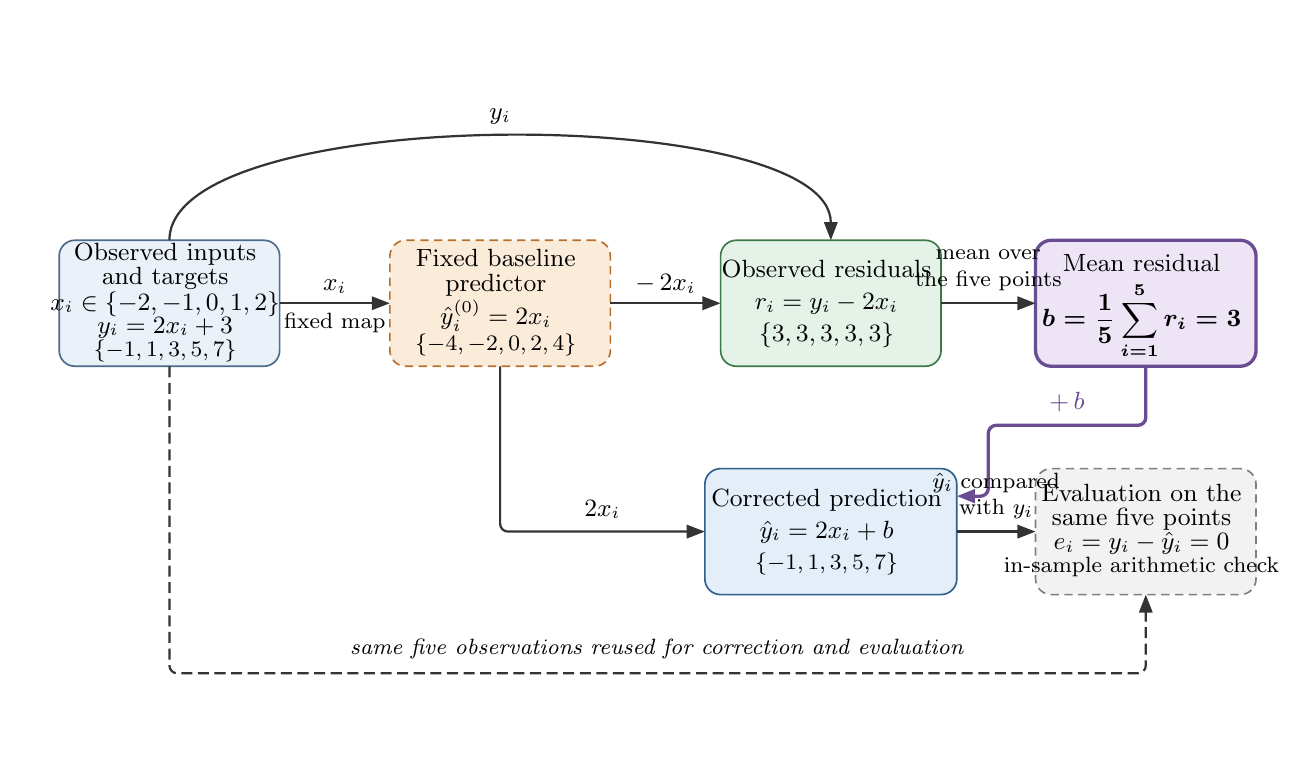
\begin{tikzpicture}[
    x=1cm,y=1cm,
    box/.style={
        rectangle,
        rounded corners=2mm,
        line width=0.6pt,
        minimum width=2.8cm,
        minimum height=1.6cm,
        inner sep=0pt,
        outer sep=0pt
    },
    flow/.style={
        draw=arrowgray,
        line width=0.8pt,
        -{Triangle[length=2.3mm,width=1.7mm]},
        rounded corners=1mm
    },
    label/.style={
        font=\small,
        inner sep=1.2pt,
        align=center
    },
    content/.style={
        font=\small,
        inner sep=0pt,
        align=center
    }
]
% White, borderless 16:9 canvas.
\path[use as bounding box] (0,0) rectangle (16,9);
\fill[white] (0,0) rectangle (16,9);

% Fixed-size node shapes.
\node[box,fill=inputfill,draw=inputedge]
    (inputs) at (1.8,5.5) {};
\node[box,fill=basefill,draw=baseedge,
      dash pattern=on 3pt off 2pt]
    (baseline) at (6.0,5.5) {};
\node[box,fill=resfill,draw=resedge]
    (residuals) at (10.2,5.5) {};
\node[box,fill=scalarfill,draw=scalaredge,line width=1.2pt]
    (scalar) at (14.2,5.5) {};
\node[box,minimum width=3.2cm,fill=predfill,draw=prededge]
    (prediction) at (10.2,2.6) {};
\node[box,fill=evalfill,draw=evaledge,
      dash pattern=on 3pt off 2pt]
    (evaluation) at (14.2,2.6) {};

% Compact Computer Modern text, kept separate from the fixed-size shapes.
\node[content] at (inputs.center) {%
    \renewcommand{\arraystretch}{0.74}%
    \begin{tabular}{@{}c@{}}
        $\text{Observed inputs}$\\
        $\text{and targets}$\\
        $x_i\in\{-2,-1,0,1,2\}$\\
        $y_i=2x_i+3$\\
        {\footnotesize $\{-1,1,3,5,7\}$}
    \end{tabular}
};
\node[content] at (baseline.center) {%
    \renewcommand{\arraystretch}{0.85}%
    \begin{tabular}{@{}c@{}}
        $\text{Fixed baseline}$\\
        $\text{predictor}$\\
        $\hat y^{(0)}_i=2x_i$\\
        {\footnotesize $\{-4,-2,0,2,4\}$}
    \end{tabular}
};
\node[content] at (residuals.center) {%
    \renewcommand{\arraystretch}{1.05}%
    \begin{tabular}{@{}c@{}}
        $\text{Observed residuals}$\\
        $r_i=y_i-2x_i$\\
        $\{3,3,3,3,3\}$
    \end{tabular}
};
\node[content] at (scalar.center) {%
    \renewcommand{\arraystretch}{1.15}%
    \begin{tabular}{@{}c@{}}
        $\text{Mean residual}$\\
        $\displaystyle\boldsymbol{b=\frac{1}{5}\sum_{i=1}^{5}r_i=3}$
    \end{tabular}
};
\node[content] at (prediction.center) {%
    \renewcommand{\arraystretch}{1.05}%
    \begin{tabular}{@{}c@{}}
        $\text{Corrected prediction}$\\
        $\hat y_i=2x_i+b$\\
        {\footnotesize $\{-1,1,3,5,7\}$}
    \end{tabular}
};
\node[content] at (evaluation.center) {%
    \renewcommand{\arraystretch}{0.74}%
    \begin{tabular}{@{}c@{}}
        $\text{Evaluation on the}$\\
        $\text{same five points}$\\
        $e_i=y_i-\hat y_i=0$\\
        {\footnotesize $\text{in-sample arithmetic check}$}
    \end{tabular}
};

% Observed inputs feed the fixed map.
\draw[flow] (inputs.east) --
    node[label,above=2pt] {$x_i$}
    node[label,below=2pt,font=\footnotesize] {$\text{fixed map}$}
    (baseline.west);

% Observed targets bypass the baseline and enter only the residual node.
\draw[flow] (inputs.north)
    .. controls (1.8,8.05) and (10.2,8.05) ..
    node[label,pos=0.5,above=3pt] {$y_i$}
    (residuals.north);

\draw[flow] (baseline.east) --
    node[label,above=2pt] {$-\,2x_i$}
    (residuals.west);

\draw[flow] (residuals.east) --
    node[label,above=3pt,font=\footnotesize]
        {$\text{mean over}$\\$\text{the five points}$}
    (scalar.west);

% The unchanged baseline prediction feeds the corrected prediction.
\draw[flow] (baseline.south) --
    (6.0,2.6) --
    node[label,above=3pt] {$2x_i$}
    (prediction.west);

% One scalar output; the route clears the evaluation box and comparison arrow.
\draw[flow,draw=scalaredge,line width=1.2pt]
    (scalar.south) --
    (14.2,3.95) --
    node[label,above=3pt,text=scalaredge] {$+\,b$}
    (12.2,3.95) --
    (12.2,3.05) --
    ($(prediction.east)+(0,0.45)$);

\draw[flow] (prediction.east) --
    node[label,above=3pt,font=\footnotesize]
        {$\hat y_i\ \text{compared}$\\$\text{with}\ y_i$}
    (evaluation.west);

% The same observations are reused for correction and evaluation.
\draw[flow,dash pattern=on 4pt off 2pt]
    (inputs.south) --
    (1.8,0.8) --
    node[midway,above=4pt,font=\footnotesize,inner sep=1pt]
        {\textit{same five observations reused for correction and evaluation}}
    (14.2,0.8) --
    (evaluation.south);

\end{tikzpicture}%
}
\end{document}